% Copyright (C) 2012 Frederik Heber, Julian Iseringhausen
% 
% This file is part of ScaFaCoS.
% 
% ScaFaCoS is free software: you can redistribute it and/or modify it
% under the terms of the GNU Lesser Public License as published by the
% Free Software Foundation, either version 3 of the License, or (at
% your option) any later version.
% 
% ScaFaCoS is distributed in the hope that it will be useful, but
% WITHOUT ANY WARRANTY; without even the implied warranty of
% MERCHANTABILITY or FITNESS FOR A PARTICULAR PURPOSE. See the GNU
% Lesser Public License for more details.
% 
% You should have received a copy of the GNU Lesser Public License
% along with this program. If not, see
% <http://www.gnu.org/licenses/>.
% 
%
\chapter{vmg -- Versatile Multigrid}
\label{cha:vmg}

\newcommand{\vmgcite}[1]{\mbox{[VMG-#1]}}

\solvertoindex{vmg}
\solvertoindex{Versatile Multigrid}
\index{Multigrid}

vmg is a grid-based solver for computing the long-range Coulomb interactions of particles for periodic boundary conditions.

\begin{figure}
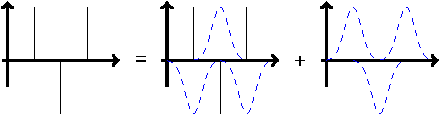
\includegraphics[width=0.9\textwidth]{figures/vmg_short-long-splitting.pdf}
\caption{The charge distribution consisting of point charges (left) is split into a smoothened part (right) and the rest (center), see~\vmgcite{1}}
\label{fig:vmg_long-short-splitting}
\end{figure}

In depth, the Coulomb problem is first split into a short-range and a long-range part, for when treated individually each can be solved efficiently. This is done by adding so-called shield charges at the same position as each point-like charge, see figure~\ref{fig:vmg_long-short-splitting}. These are described by a spline function that has compact support, is symmectric around its center and is normalized to the same magnitude as the original point-like charge. The short-range part (center,  fig.~\ref{fig:vmg_long-short-splitting}) is then solved by a direct summation of the pair-wise interactions between the small number of charges lying in the compact support of these shield charges. Outside of the support, shield charge and oppositely charged point-like charge precisely cancel. The long-range part consists of the potential induced by these shield charges. It is treated by solving a well-known partial differential equation (PDE) in the form $Lu=f$, the Poisson equation, where $L$ is the negated Laplace operator $L:=-\Delta$, $u$ is the sought-for solution and $f$ is the "right-hand side", i.\,e.~the shield charges sampled on the grid.

Solving PDEs numerically is usually done by discretizing their differential operator in an extension of the idea of calculating a derivative via the method of finite differences. This converts the continuous problem $Lu=f$ into a discrete problem $Ax=b$, where $A$ is the matrix of the discretized operator, $x$ is the discrete solution and $b$ is again the "right-hand side". In the multigrid ansatz, see~\vmgcite{2}, $Ax=b$ is obtained on the finest grid (of $d$ dimensions) while on coarser grids the so-called defect equation $Ax^\prime=b-Ax$ is solved. This offers the advantage that the solution time is independent of the system size. The basic idea of a multigrid is to eliminate the residual, i.\,e.~the error $(b-Ax)$, at each coarser and coarser level. The picture to have in mind is that the "noise" is reduced at multiple frequencies at the same time. 

A cycle of two grids, i.\,e.~a fine grid and a coarser one, then consists of steps of "removing noise" (smoothing), projecting down onto the coarser grid (restriction), solving exactly and bringing this solution back onto the finer grid (prolongation). A multigrid cycle then consists of the recursive application of two-grid cycles instead of solving exactly, i.\,e.~we step down the grid hierarchy from a finer to the next coarser grid and eventually move up again.

There are many types of this cycle differing in the precise sequence of smoothing, prolongation, and restriction steps. Since this is an iterative process we have to perform such a cycle a (typically small) number of times until the residual is small enough. Then we have "converged" sufficiently to the solution.

In order to set up the above PDE, we need the right-hand side $b$ that consists of the aforementioned shield charges. After solving the PDE on the grid, the Coulomb potential at the charge positions is obtained by some interpolation scheme. Right now, a multidimensional Newton interpolation is used, see \vmgcite{3}, where a polynomial is fit to the solution around the desired position. The field is calculated via analytical differentiation of these polynomials.

To sum it all up, the multigrid does the following:
\begin{enumerate}
 \item Bring the shield charges onto the grid (the right-hand side) by evaluating spline functions for each particle charge.
 \item Iterate over the multigrid in a specific cycle until either the (absolute or relative) residual is lower than a given threshold value (converged) or a set maximum number of iterations steps is reached (non-converged).
 \item The solution is interpolated back at the position of each charge, yielding the long-range interactions.
 \item Short-range interactions are determined via direct summation.
\end{enumerate}

Crucial for its accuracy are then the following parameters of the multigrid solver:
\begin{description}
 \item[grid size] This determines the number of grid points per axis on the finest level. This parameter mainly affects the accuracy of the long-range part of the solution.
 \item[width of spline support] This gives the width of the shield charges. The greater is the width, the more accurate the solution becomes, but at the same time the more interactions have to be evaluated with the (computationally expensive) short-range part of the solver. One has to ensure that the number of particles in the support of these shield charges is kept constant, otherwise the algorithm does not scale optimally anymore.
 \item[discretization scheme] This is the manner of constructing a matrix $A$ from the continuous Laplace operator $L$. A scheme of higher order gives greater accuracy w.r.t. a fixed grid size. This parameter is solely affecting the accuracy of the long-range part of the algorithm.
\end{description}

For parallelization the particles are distributed over many processes. Each brings its local particles onto the grid. Also, each process has a certain share of the grid and performs its multigrid operations on its share, communicating with neighboring processes during the restriction, prolongation, and smoothing. Conceptionally, there is also one global communication in every multigrid iteration where the local residuals get summed up globally. Eventually, each process interpolates back its particle potential.

\section*{Common capabilities}

\begin{description}

  \item[Periodicity:]
Currently only periodic boundary conditions are supported. Support for open or mixed boundary conditions is in progress.

  \item[Box shape:] Cubic boxes are supported.
  
  \item[Tolerances:] ?

  \item[Delegate near-field:] Not implemented.

  \item[Virial:] No.

\end{description}

\section*{Additional capabilities}

 Due to the aforementioned splitting of the Coulomb interactions into a short- and a long-range part, some parameters affect only the accuracy of either and not necessarily of both, see their desription. If then a system only has a small long-range part, one may save substantial calculation time by decreasing accuracy specifically for long-range calculations. This allows checking whether either interactions part far outweighs the other.
 Via the configure switch \emph{--enable-debug-output} the various energy contributions of short- and long-range parts are printed to the console. Note however that this switch should \emph{not be used for production runs} as it makes unnecessary additional calculations once an efficient set of parameters has been found.

% \begin{description}

% \end{description}

\section*{Solver specific functions}

\begin{itemize}

  \item
\begin{alltt}
fcs\_vmg\_set\_max\_level(FCS handle, fcs_int max_level);
\end{alltt}
Sets the number of points per axis of the finest grid (optional,default=6).
More specifically it is $2^{\text{max\_level}}$, i.e. more points means better approximated solution but scales with ${\cal O}(\text{max\_level}^3)$. This is the first value to change for better accuracy, see also near\_field\_cells.
  \item
\begin{alltt}
fcs\_vmg\_get\_max\_level(FCS handle, fcs\_int* max\_level);
\end{alltt}
Get the maximum level of the multigrid algorithm.

  \item
\begin{alltt}
fcs\_vmg\_set\_max\_iterations(FCS handle, fcs\_int max\_iterations);
\end{alltt}
Sets the maximum number of multigrid iterations (optional, default=15).
This is the second threshold besides \emph{precision} that will stop the iteration. Normally, you don't need to change this value, this is only present in case the iteration does not converge and this sets after how many iteration steps it is considered as "not converged".

  \item
\begin{alltt}
fcs\_vmg\_get\_max\_iterations(FCS handle, fcs\_int* max\_iterations);
\end{alltt}
Get the maximum number of multigrid iterations.

  \item
\begin{alltt}
fcs\_vmg\_set\_smoothing\_steps(FCS handle, fcs\_int smoothing\_steps);
\end{alltt}
Set the number of smoothing steps in the multigrid cycle per level (optional, default=3).
Smoothing refers to removal of error at a certain level. This is usually done for a fixed and small number of iterations. Usually, there is no need to change it. Fewer steps may be faster (and may cause solution not to converge anymore). Does not affect the precision but only the computational efficiency.

  \item
\begin{alltt}
fcs\_vmg\_get\_smoothing\_steps(FCS handle, fcs\_int *smoothing\_steps);
\end{alltt}
Get the number of pre/post-smoothing steps on each level.

  \item
\begin{alltt}
fcs\_vmg\_set\_cycle\_type(FCS handle, fcs\_int cycle\_type);
\end{alltt}
Specifies the type of multigrid cycle, 1 V-cycle, 2 W-cycle, \ldots (optional, default=1).
For parallel computation, V-cycle is the correct type, for serial computation W-cycle might be slightly more efficient. In case of doubt, leave it to default.

  \item
\begin{alltt}
fcs\_vmg\_get\_cycle\_type(FCS handle, fcs\_int *cycle\_type);
\end{alltt}
Get the cycle\_type-number of the multigrid cycle used.

  \item
\begin{alltt}
fcs\_vmg\_set\_precision(FCS handle, fcs\_float precision);
\end{alltt}
Set the threshold for (absolute and relative) residual below which internal iteration is stopped (optional, default=1.0e-8).
This is not equal to FCS's global tolerance! As an estimate one might use one magnitude below desired tolerance.

  \item
\begin{alltt}
fcs\_vmg\_get\_precision(FCS handle, fcs\_float *precision);
\end{alltt}

  \item
\begin{alltt}
fcs\_vmg\_set\_near\_field\_cells(FCS handle, fcs\_int near\_field\_cells);
\end{alltt}
Set the half witdh in number of grid points of compact local support of b-spline function (radius of shielding charges) (optional, default=4).
This value along with max\_level has great impact on accuracy but the correlation is reciprocal.

  \item
\begin{alltt}
fcs\_vmg\_get\_near\_field\_cells(FCS handle, fcs\_int *near\_field\_cells);
\end{alltt}
Get the number of near field cells for separating the near/far field part of the potential.

  \item
\begin{alltt}
fcs\_vmg\_set\_interpolation\_order(FCS handle, fcs\_int interpolation\_order);
\end{alltt}
Set polynomial order of tensored Newton back-interpolation of solution at the site of each charge (optional, default=5).
Usually, does not need to be changed. Normally, less means precision of grid solution is omitted, more means useless computation.

  \item
\begin{alltt}
fcs\_vmg\_get\_interpolation\_order(FCS handle, fcs\_int *interpolation\_order);
\end{alltt}
Get the interpolation order for interpolating the gridded potential to the particle positions.

  \item
\begin{alltt}
fcs\_vmg\_set\_discretization\_order(FCS handle, fcs\_int discretization\_order);
\end{alltt}
Discretization scheme in setting up partial differential equation (optional, [2,4], default=4).
This heavily influences precision of solution in conjunction with near\_field\_cells ans max\_level. This parameter enables direct control of the discretization error of the long-range part. Default is 4 and leave it at that.

  \item
\begin{alltt}
fcs\_vmg\_get\_discretization\_order(FCS handle, fcs\_int *discretization\_order);
\end{alltt}
Get the order of the discretization scheme.

\end{itemize}

\section*{Known bugs or missing features}

\begin{itemize}
  \item Open and mixed boundaries still need to be incorporated.
  \item Separate near-field part?
  \item How to compute the virial?
\end{itemize}

\paragraph{References}
\todo[inline]{move vmg citations to bibliography}
\begin{footnotesize}
\begin{itemize}
  \item[vmg-1] M.~Griebel, S.~Knapek, G.~Zumbusch \textbf{Numerical Simulation in Molecular Dynamics -- Numerics, Algorithms, Parallelization, Applications}, 2007
  \item[vmg-2] U.~Trottenberg, C.~W.~Oosterlee, A.~Schuller \textbf{Multigrid}, 2000
  \item[vmg-3] K.~A.~Atkinson \textbf{Introduction to Numerical Analysis}, 1988
\end{itemize}
\end{footnotesize}


%%% Local Variables: 
%%% mode: latex
%%% TeX-master: ug.tex
%%% End: 


%%% Local Variables: 
%%% mode: latex
%%% TeX-master: ug.tex
%%% End: 

